\pdfoutput=1
\documentclass{JINST}
\let\ifpdf\relax

\usepackage{epsfig}
\usepackage{subfigure}
\usepackage{wrapfig}
\usepackage{multirow}

\title{Parallel Computing and the Search for Jets and Black Holes at the LHC}

\author{V. Halyo\thanks{Corresponding Author}, P. LeGresley, P. Lujan \\
\llap Princeton University, Princeton, NJ, USA \\
E-mail: \email{vhalyo@gmail.com}}

\abstract{Massively parallel computing architecture at the LHC could be the necessary leap to
an era of new discoveries at the LHC following the Higgs like particle in 2012.
Scientific computing constitute an essential part of LHC experiment. It takes part in the
operation,Trigger,  LHC GRID, simulation and analysis. 
The flexibility of the trigger system and the quest for new physics at the LHC suggest
the High Level trigger to be the first place to integrate GPU/MIC hardware in its 
commercial computer farms.

This cutting edge technology provides the architecture not only to accelerate 
existing algorithms but also the opportunity to develop new algorithms that select events 
that could have evaded detection previously. In this article we describe
new algorithms to select prompt or non prompt  jets and black holes in the silicon tracker.
}
\keywords{ATLAS; CMS; Level-1 trigger; HLT; Tracker system; Jets; Black holes}

\begin{document}

\section{Introduction} 

Data analysis at the LHC requires approaches to processing that are effective at finding the underlying physics phenomena while still being cost efficient.  Using computing technologies derived from consumer products results in lower hardware acquisition costs because many of the research, development, and manufacturing costs are amortized over much larger volumes.  These consumer products are increasingly mobile devices such as phones, tables, and notebook computers so there is significant interest in energy efficiency to maximize battery life.  This focus on energy efficiency also the potential to benefit more traditional areas of computing and data analysis by reducing operating costs such as electrical power and cooling.

Leveraging processors derived from consumer products helps minimize costs associated with purchasing and operating large compute installations such as required for the LHC, but there is also a software aspect that needs to be considered.  Moore's Law continues to yield ever more powerful processors but the architecture of processors has changed significantly over the past decade.  For many years CPUs were able to run the exact same software faster and faster with each new generation of processor.  This changed in the early 2000s as Intel and AMD shifted focus to multicore processors featuring at first two cores, but with some newer processors featuring as many as 16 cores.

Parallel processors, in the form of multicore CPUs and more recently highly programmable Graphics Processing Units (GPUs), may require a significant rethink of algorithms and their implementations.  At the same time the High Energy Physics (HEP) community is at a crossroads with tentative confirmation of the Higgs particle completing the search for particles predicted by the Standard Model.  The search for physics beyond the Standard Model will require development of advanced algorithms for detecting rare new physics phenomena, and these new algorithms will need to be designed and implemented based on knowledge of the current state and likely future directions for processor architecture.

\section{Physics Motivation}


Various extensions Beyond the Standard Model (BSM) predict the existence of new, strongly interacting particles that lead to final states
with high jet multiplicities. Other exotic models might include boosted jets or long-lived neutral particles decaying
at macroscopic distances from the primary vertex~\cite{bib:hiddenvalley} in the tracker. The key to observe these events is to be
able to select these jets in real time in the trigger system.

Both CMS~\cite{Chatrchyan:2008aa} and ATLAS~\cite{Aad:2008zzm} have a typical trigger system with a hierarchy of multiple levels, 
ranging from fast and relatively simple criteria implemented entirely in hardware and firmware, to more sophisticated software-based analysis. 
The primary goal of the software based level is to apply a specific set of 
physics selection algorithms on the events read out and accept the events with the most interesting physics 
content. This computationally intensive processing is executed on a farm of commercial CPU processors.
The quest for new physics and the flexibility of the trigger system suggest that this computer farm is the natural
place to integrate GPU or MIC cards. These cards allow to develop fast and unique algorithms using Massively parallel programming architecture
to select events that clearly smoking gun to physics BSM. 

In this article we would describe newly developed trigger algorithms that would be able to select events
that include displaced jets originating from long lived particles, or various topologies with boosted jets that will
be more frequent as the center of mass energy of the collision at design luminosity is increased. These new
triggers will naturally be sensitive to a larger parameter space, including lower-mass Higgs that decay to
displaced heavy flavor hadrons, that could have evaded detection in previous experiments. For example, CMS has 
performed a search for long-lived neutral particles decaying to displaced leptons~\cite{Chatrchyan:2012jna}, 
but the efficiency for measuring leptons originating from a low-mass Higgs of $M_H = 120$ GeV/$c^2$ is very low 
due to the lepton momentum requirements in the trigger, resulting in relatively poor limits for this mass region.

Generalization of the trigger algorithm we develop in this article would allow us to search for 
 the existence of soft displaced black hole like decay. Namely, high multiplicity democratic decay of soft particles  
that originate few centimeter from the interaction point. To conclude, 
introducing parallel programming allows to develop algorithms that are not CPU expensive and
might provide us an invaluable way to test any topological signature that clearly does not exist in the SM.



\section{Processor Architecture}

When discussing computer processors it is common to bring up Moore's Law.  However, it is important to recognize what Moore's Law actually represents.  Moore's Law is an empirical observation made by Intel co-founder Gordon Moore in the 1960s that it was economically feasible to double the number of transistors on a single integrated circuit every 24 months.  So although modern usage tends to associate Moore's Law with processor performance it is first and foremost about manufacturing technology and the ability to fabricate ever smaller transistors.

In terms of performance, one of the most obvious benefits of smaller transistors is the ability to run processors at faster clock rates.  Over the course of a few years processor clock speeds jumped from tens of MHz to GHz speeds.  However, manufacturers were not able to fully decrease operating voltages in a corresponding way and this led to increases in power density and the inability to dissipate so much power from such a small area.  For the first time processors had become power limited.

It is fairly clear how a faster clock speed yields a faster processor.  What is a little less obvious is how more transistors can make a single core processor faster even at fixed clock speeds.  One option is to perform multiple operations at each clock cycle with parallel execution units.  In the late 1990s Intel and AMD added something to their processors that has come to be known as SSE, or Streaming SIMD Extensions, where SIMD refers to a type of parallel architecture as defined by Flynn's taxonomy.  In the SIMD (Same Instruction Multiple Data) model one instruction such as multiplication, addition, etc. is applied to multiple data items.  For example, if one wanted to add together two vectors the most obvious approach is to add the first elements from each vector together, then the second elements, and so on.  With SSE one would use one instruction to add together the first $n$ elements from each vector, where the value of $n$ depends on the data type and the width of the SSE units.  Then one would add the next $n$ elements and so on until the full vector has been processed.  In this approach the parallelism is to be expressed by the software developer based on the computations to be performed and the capabilities of the hardware.  Most modern compilers can also target the SSE units in a process typically referred to as auto vectorization.  The effectiveness of auto vectorization depends on the capabilities of the compiler, the complexity of the code being analyzed, and the skill of the software developer at writing code that can be successfully analyzed by the compiler.

A potential disadvantage of the SSE approach is that it requires software that specifically makes use of it, either through manual programming by the software developer or auto vectorization at compile time.  But the additional transistors available at each generation of Moore's Law also allowed hardware designers to implement Instruction Level Parallelism (ILP).  Instead of the processor executing one operation per clock cycle (an arithmetic operation, a load from memory, a store back to memory, etc.) multiple instructions are executed in parallel.  For example, a load from memory is issued for a future arithmetic operation, an arithmetic operation is performed, and a store back to memory of a previous arithmetic operation is issued.  In x86 processors this hardware is determined dynamically as the program is executing and allows arbitrary single-threaded software to run faster by exploiting parallelism within the instruction stream.

The implementation of ILP and the associated techniques of instruction pipelining, out-of-order execution, speculative execution, and hardware branch prediction helped consume many of the additional transistors made available through Moore's Law.  But in addition to ILP, the growing gap between the performance of the processors running at GHz speeds and the off chip memory systems necessitated adding a complicated cache hierarchy to modern processors.

While compute performance may increase around 40\% per year in accordance with Moore's Law, memory performance increases approximately 10\% year.  If left unchecked this gap in performance would have resulted in processors that had the potential to be very computationally powerful but would be limited in actual performance because of the constant need to wait on the memory system.  To address this modern processors have a complicated cache hierarchy not only for data, but also for instructions, and even for translating virtual memory addresses to physical memory addresses in the form of Translation Lookaside Buffers (TLB).  Additional logic in the form of hardware prefetchers observes memory access patterns in real time and attempts to prefetch into the caches data and instructions that are likely to be needed in the future.  The disparity between processor and memory performance is so bad that the vast majority of the processor is devoted not to computation but to data handling.  As shown in Figure~\ref{fig:core_i7_die} the L3 cache plus the memory controller and other I/O portions of a chip can easily represent around 50\% of the area.  Within each core there is an L1 and L2 cache, plus all of the logic associated with ILP for that core.  The actual chip area devoted to computations is remarkably small.

\begin{figure}[!Hhtb]
\begin{center}
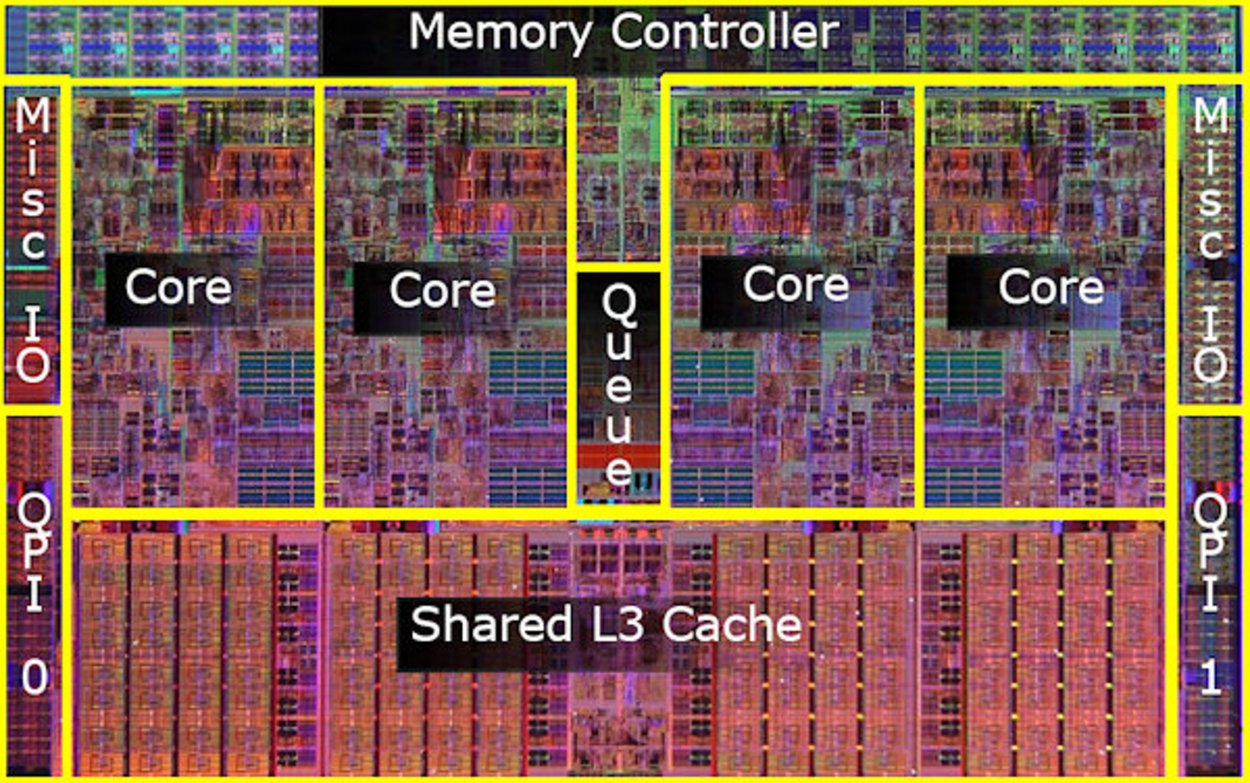
\includegraphics[width=0.75\textwidth]{figs/Core_i7_die.pdf}
\caption{Intel Core i7 die showing major components of the processor (image from Intel). \label{fig:core_i7_die}}
\end{center}
\end{figure}

Faster clock speeds, ILP, and hardware prefetechers had the advantage of using existing software and simply running it faster.  However, there are limits to what the hardware can do to automatically extract ILP and predict the memory access pattern of arbitrary applications.  Deep instruction pipelines, which in some processors exceeded 30 stages, have issues with hazards that would affect the correctness of results if not correctly handled by the processor, stalls due to unavailable inputs, and mispredicted branching behavior.  At some point this reaches a level of diminishing returns where the hardware complexity, and hence cost, outweighs the benefits.

With faster clock speeds not feasible and ILP also reaching its limits, hardware designers in the early 2000s turned to multicore to utilize all of those additional transistors available to them from Moore's Law.  As seen in Figure~\ref{fig:core_i7_die}, the hardware designers develop the design for a core, plus the hardware logic to link them together, and can then place as many cores on a single chip as current manufacturing technology allows.  With multiple cores, independent instances of applications (web browser, word processor, anti-virus, etc.) can run in parallel on the multiple cores without application level changes.  But if one application such as a video transcoder wants to speed up the processing of a video it must be specially written to make use of multiple cores.

Modern CPUs with ILP, SIMD units, and multicore are highly parallel processors yet still retain the ability to efficiently run single-threaded, sequential software because so many applications make little to no use of parallel computing.  An alternate approach would be to design an inherently parallel processor that is only designed to run parallel programs efficiently.  Such a processor would not need to run single-threaded, sequential software and therefore could devote more chip area to computations and less to features like ILP, caches, and hardware prefetechers.  An example of a processor that is specialized to running parallel workloads is GPUs.

As implied by the name GPUs were designed as specialized processors for processing graphics.  In the 1990s the initial GPUs targeted towards consumer applications handled the computations associated with computing the color of each pixel in a process referred to as pixel shading.  Like any integrated circuit, GPUs also take advantage of Moore's Law.  The pixel shaders became more programmable so that game designers could create better looking graphics that were not the same as the graphics from everyone else, and additional functionality in the form of vertex shaders were added to the GPU for processing the geometry used in 3D graphics.

CPUs are designed to be multipurpose and run operating systems, word processors, spreadsheets, games, etc. while the GPU was more special purpose and only intended to do graphics computations.  Because the GPU was intended for a specialized workload, the designers had a choice when using additional transistors to make the GPU more powerful.  One option would be to follow the CPU model and create one or more very complicated cores with ILP, caches, etc. or design a simpler, smaller core that allows many more cores per chip.  The disadvantage of simpler, smaller cores is that such a core probably won't be as fast at running single threaded code but that did not matter for the GPU since it targeted a special application area with lots of available parallelism.  Modern GPU designs use the simpler, smaller core approach and modern high end hardware has thousands of parallel execution units.

In addition to making GPUs more computationally powerful, the programmability has been improved through both changes in hardware and new software tools.  The programmability of GPUs using options such as CUDA, OpenCL, and OpenACC make the hardware usable for many applications beyond graphics, and without requiring programmers to have a specialized graphics background.  However, a strong background in parallel computing is still required to make effective use of a GPU.

With the growing success of GPUs as a massively parallel processor well suited to more general purpose applications, Intel has introduced a line of products marketed as Xeon Phi.  The Xeon Phi products physically look similar to a GPU in that they plug into a host system via PCI Express.  And from an architecture perspective they also have many similarities to GPUs.  Xeon Phi is based on an x86 Pentium core from the early 1990s.  This is a much simplified, and hence smaller, core compared to modern x86 CPUs.  To make these simplified cores more computationally powerful, 512 bit wide SIMD units known as Advanced Vector extensions 2 (AVX2) have been added to the core.  Because of the simple nature of the core, without features such as out of order execution, a single Xeon Phi processor may have up to 64 cores.

Regardless of whether the future is GPUs or the architecturally similar Xeon Phi, it seems clear that the future of computing is massively parallel processors.  This will require rethinking algorithms and their implementations to make effective use of these highly parallel processors.  Algorithms that have been viewed as computationally infeasible should be revisited, and current algorithms that do not parallelize well will need to be reworked to take advantage of modern processors.

\section{Hough Transform Algorithm}

As an example of implementing a computationally intensive algorithm on a massively parallel processor the authors have previously developed an implementation of the Hough transform using CUDA.  The Hough transform is an image processing algorithm for feature detection that considers all possible instances of a feature (line, circle, etc.).  Each possible instance of a feature starts with zero votes in the parameter space, and then for each piece of input data votes are added to the feature instances that would include that input data.  After all input data has been processed the votes in the parameter space are processed.  Locations in the parameter space with more votes are likely to be actual features in the input data so this step amounts to looking for local maxima in the parameter space.  Once candidate features have been identified more expensive computations can be applied to confirm the existence of the feature.

\begin{figure}[!Hhtb]
\begin{center}
  \subfigure[]{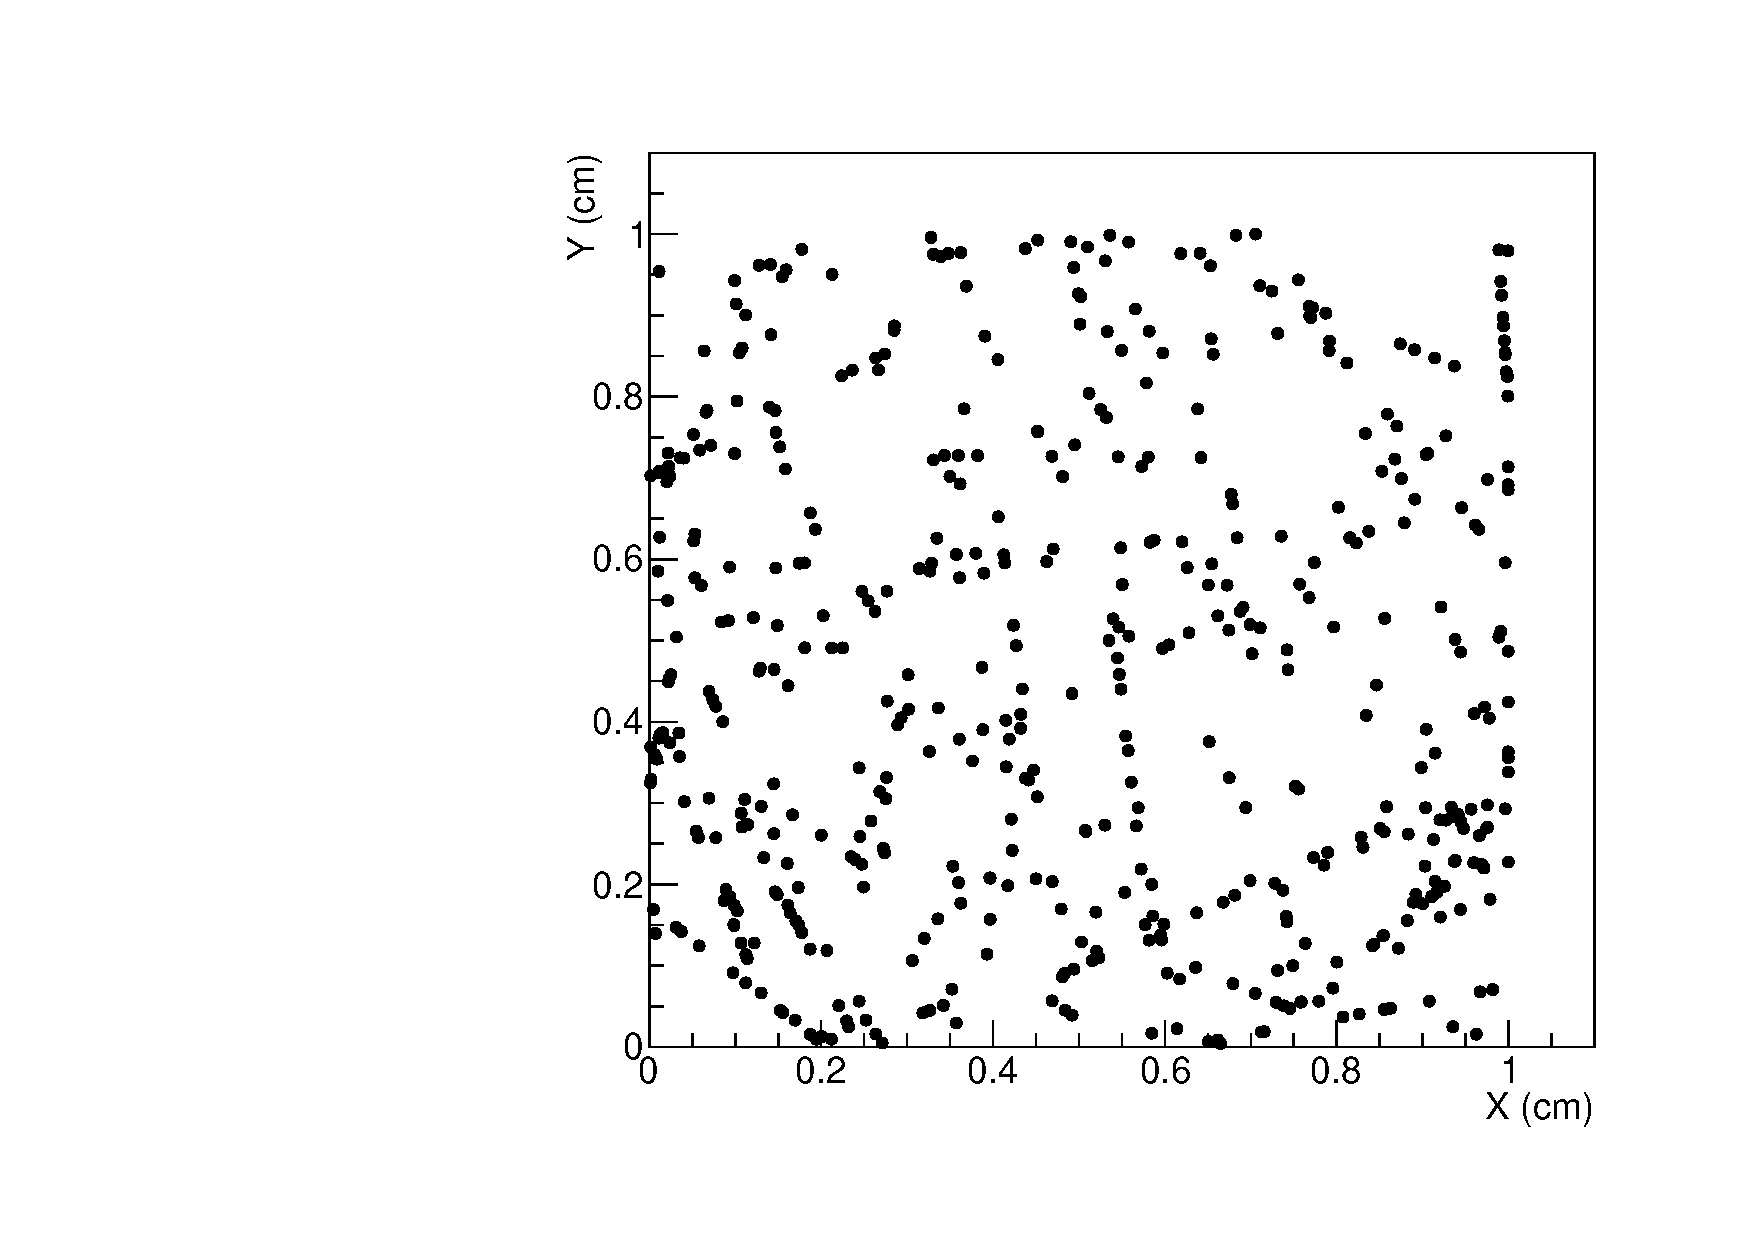
\includegraphics[width=0.32\textwidth]{figs/50events_hits.pdf} \label{fig:hits}}
  \subfigure[]{\includegraphics[width=0.30\textwidth]{figs/50events_accumulator.pdf} \label{fig:accumulator}} 
  \subfigure[]{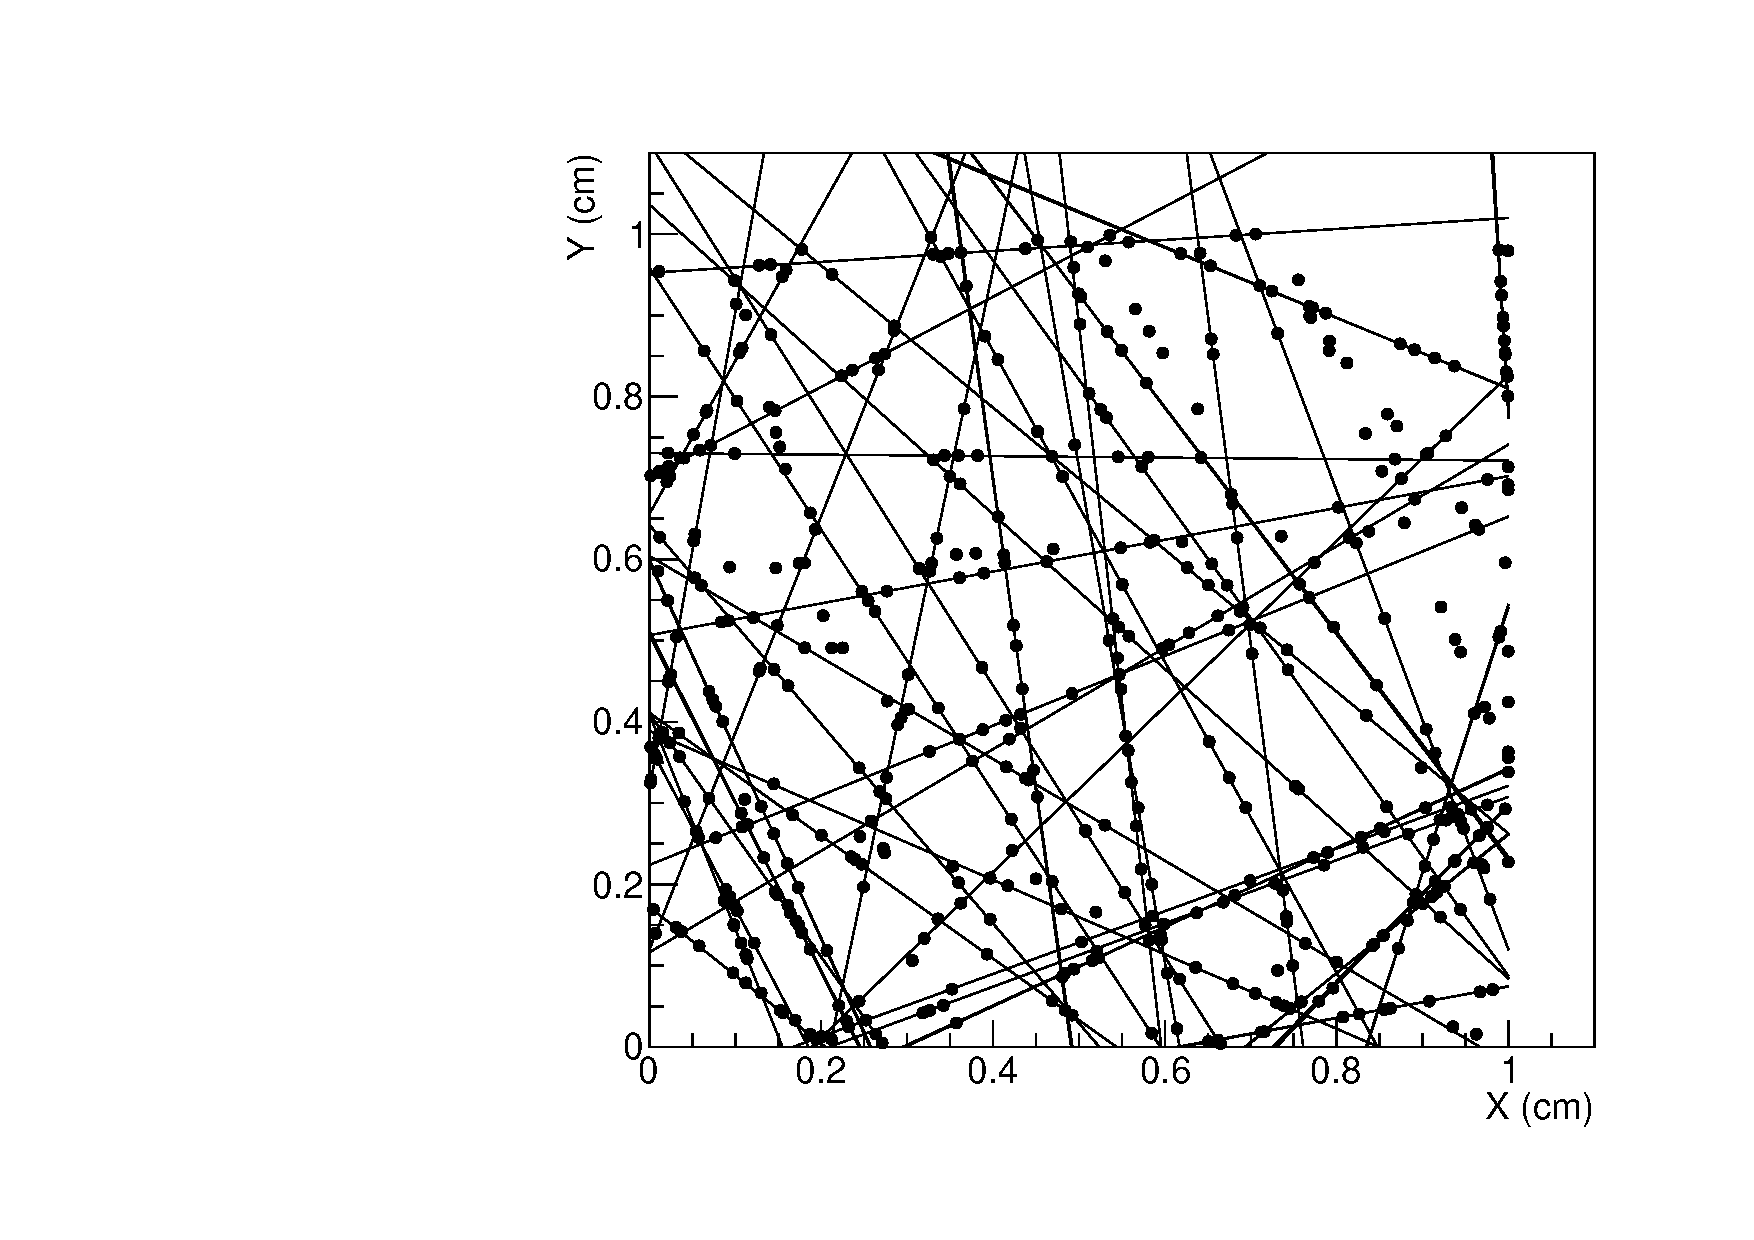
\includegraphics[width=0.32\textwidth]{figs/50events_hits_tracks.pdf} \label{fig:tracks}}
  \caption{Hough transform algorithm applied to a simple example. Left: Hits in a simulated event with 50
    straight-line tracks and 10 hits per track. Center: Each hit results in a sinusoidal curve of votes in parameter
    space. Locations with many votes are likely to be tracks in the original data. Right:
    Candidate tracks identified from finding local maxima in the parameter space.\label{fig:hough}}
\end{center}
\end{figure}

One advantage of the Hough transform is that it is tolerant to missing data or data that does not exactly fit the candidate features.  This could occur if there is noise in the data, or if the resolution of the data results in features that cannot be perfectly represented with a given computational discretization.  The downside of this robustness is that the Hough transform is computationally expensive.  However, the implementation using the GPU has demonstrated significant performance advantages compared to a multithreaded CPU implementation.  This performance comparison was made using a self developed CPU implementation because typical implementations such as the one in Intel MKL are sequential implementations that do not utilize multicore CPUs.  It was felt that the multithreaded CPU implementation was a more fair way to compare performance, but self implementations can sometimes be biased.  Therefore, additional CPU performance optimizations have been implemented in the form of using AVX intrinsics and improvements to the OpenMP parallelization.  As shown in Figure~\ref{fig:TimePerformance} the combination of improvements resulted in approximately a 40\% decrease in the runtime for the CPU implementation.

\begin{figure}[!Hhtb]
\begin{center}
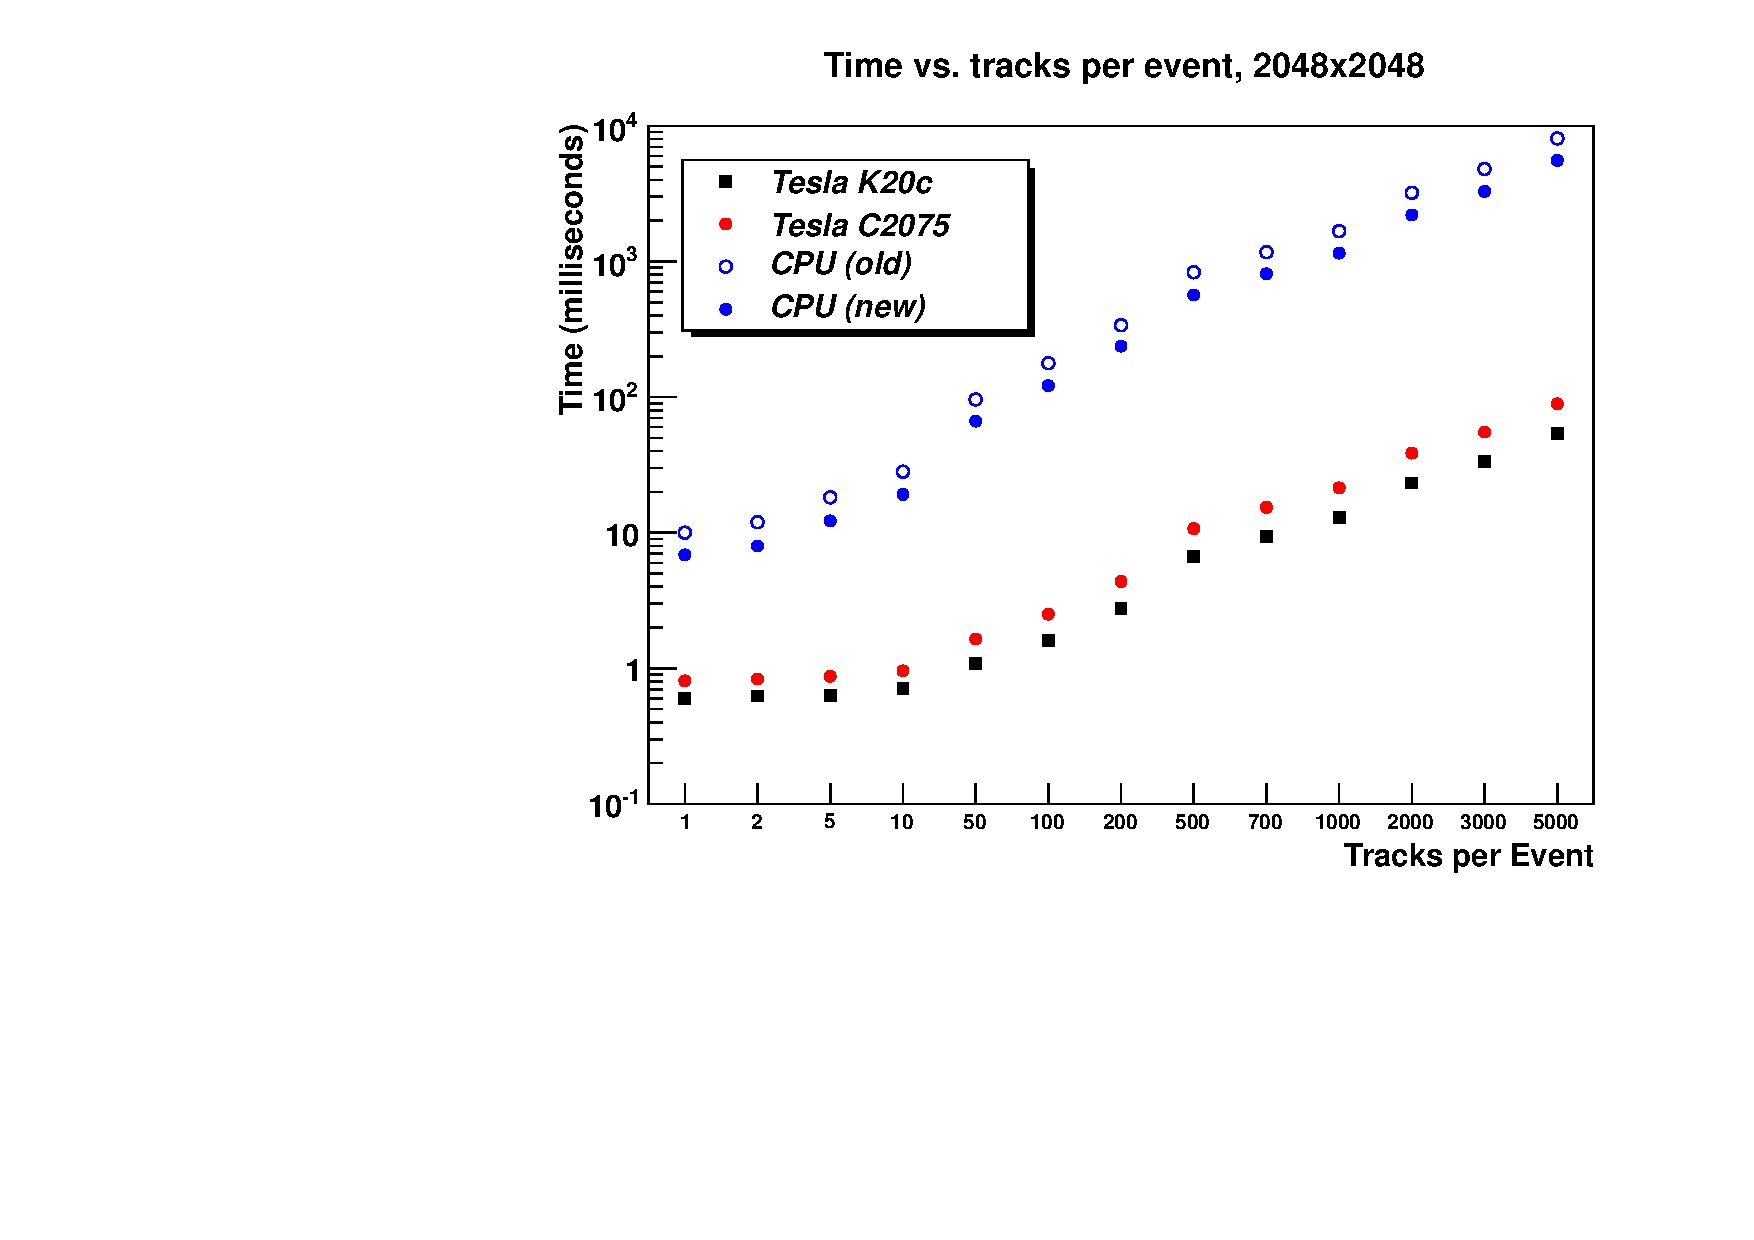
\includegraphics[width=0.75\textwidth]{figs/TimePerformance.pdf} 
\caption{Time performance of old and new CPU implementations compared to NVIDIA Tesla C2075 and K20c.  Intel Core i7-3770 CPU running a multithreaded implementation.\label{fig:TimePerformance}}
\end{center}
\end{figure}

It is worth mentioning that while the use of AVX has the potential for an 8x improvement when using single precision floating point, only improving the performance by 40\% was not unexpected for this code.  That is because the previous CPU implementation sought to minimize expensive computations by ensuring that redundant computations were moved outside of loops and intermediate results reused where possible.  These existing optimizations meant the implementation was limited more by memory access operations rather than the computational rate.  It is always useful to understand what aspect(s) of the hardware, such as computations or data access, limit the performance of an algorithm so that time spent on implementing optimizations is used effectively.

\section{Jet and Black Hole Detection}

Computational approach: two HT


\begin{figure}[!Hhtb]
\begin{center}
	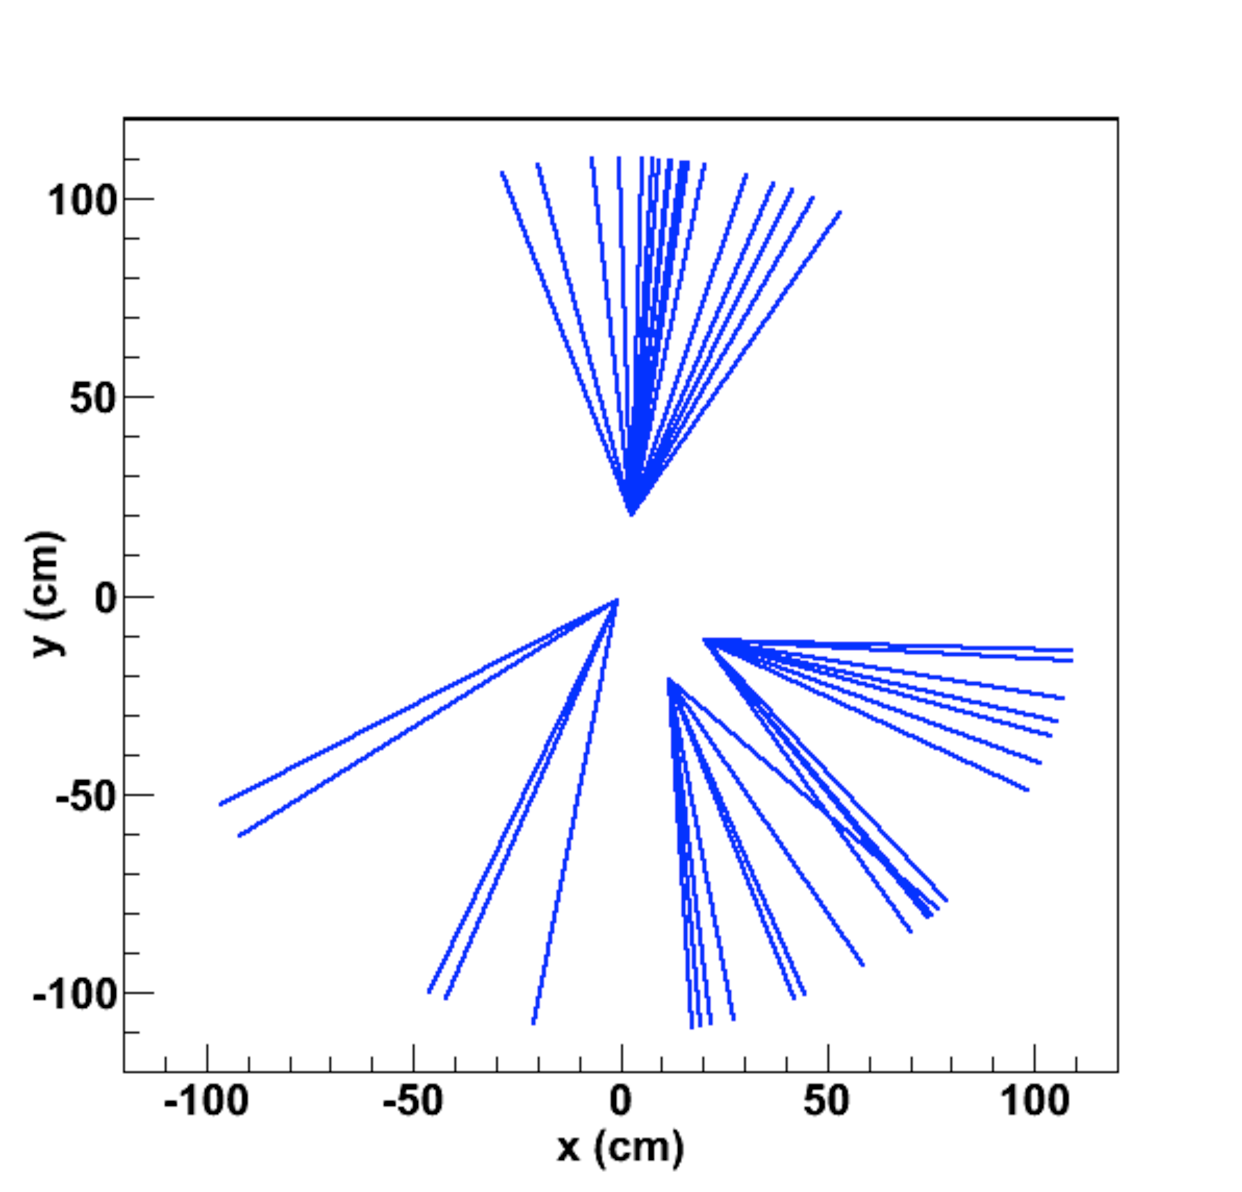
\includegraphics[width=0.35\textwidth]{figs/jet2/tracks.pdf}
	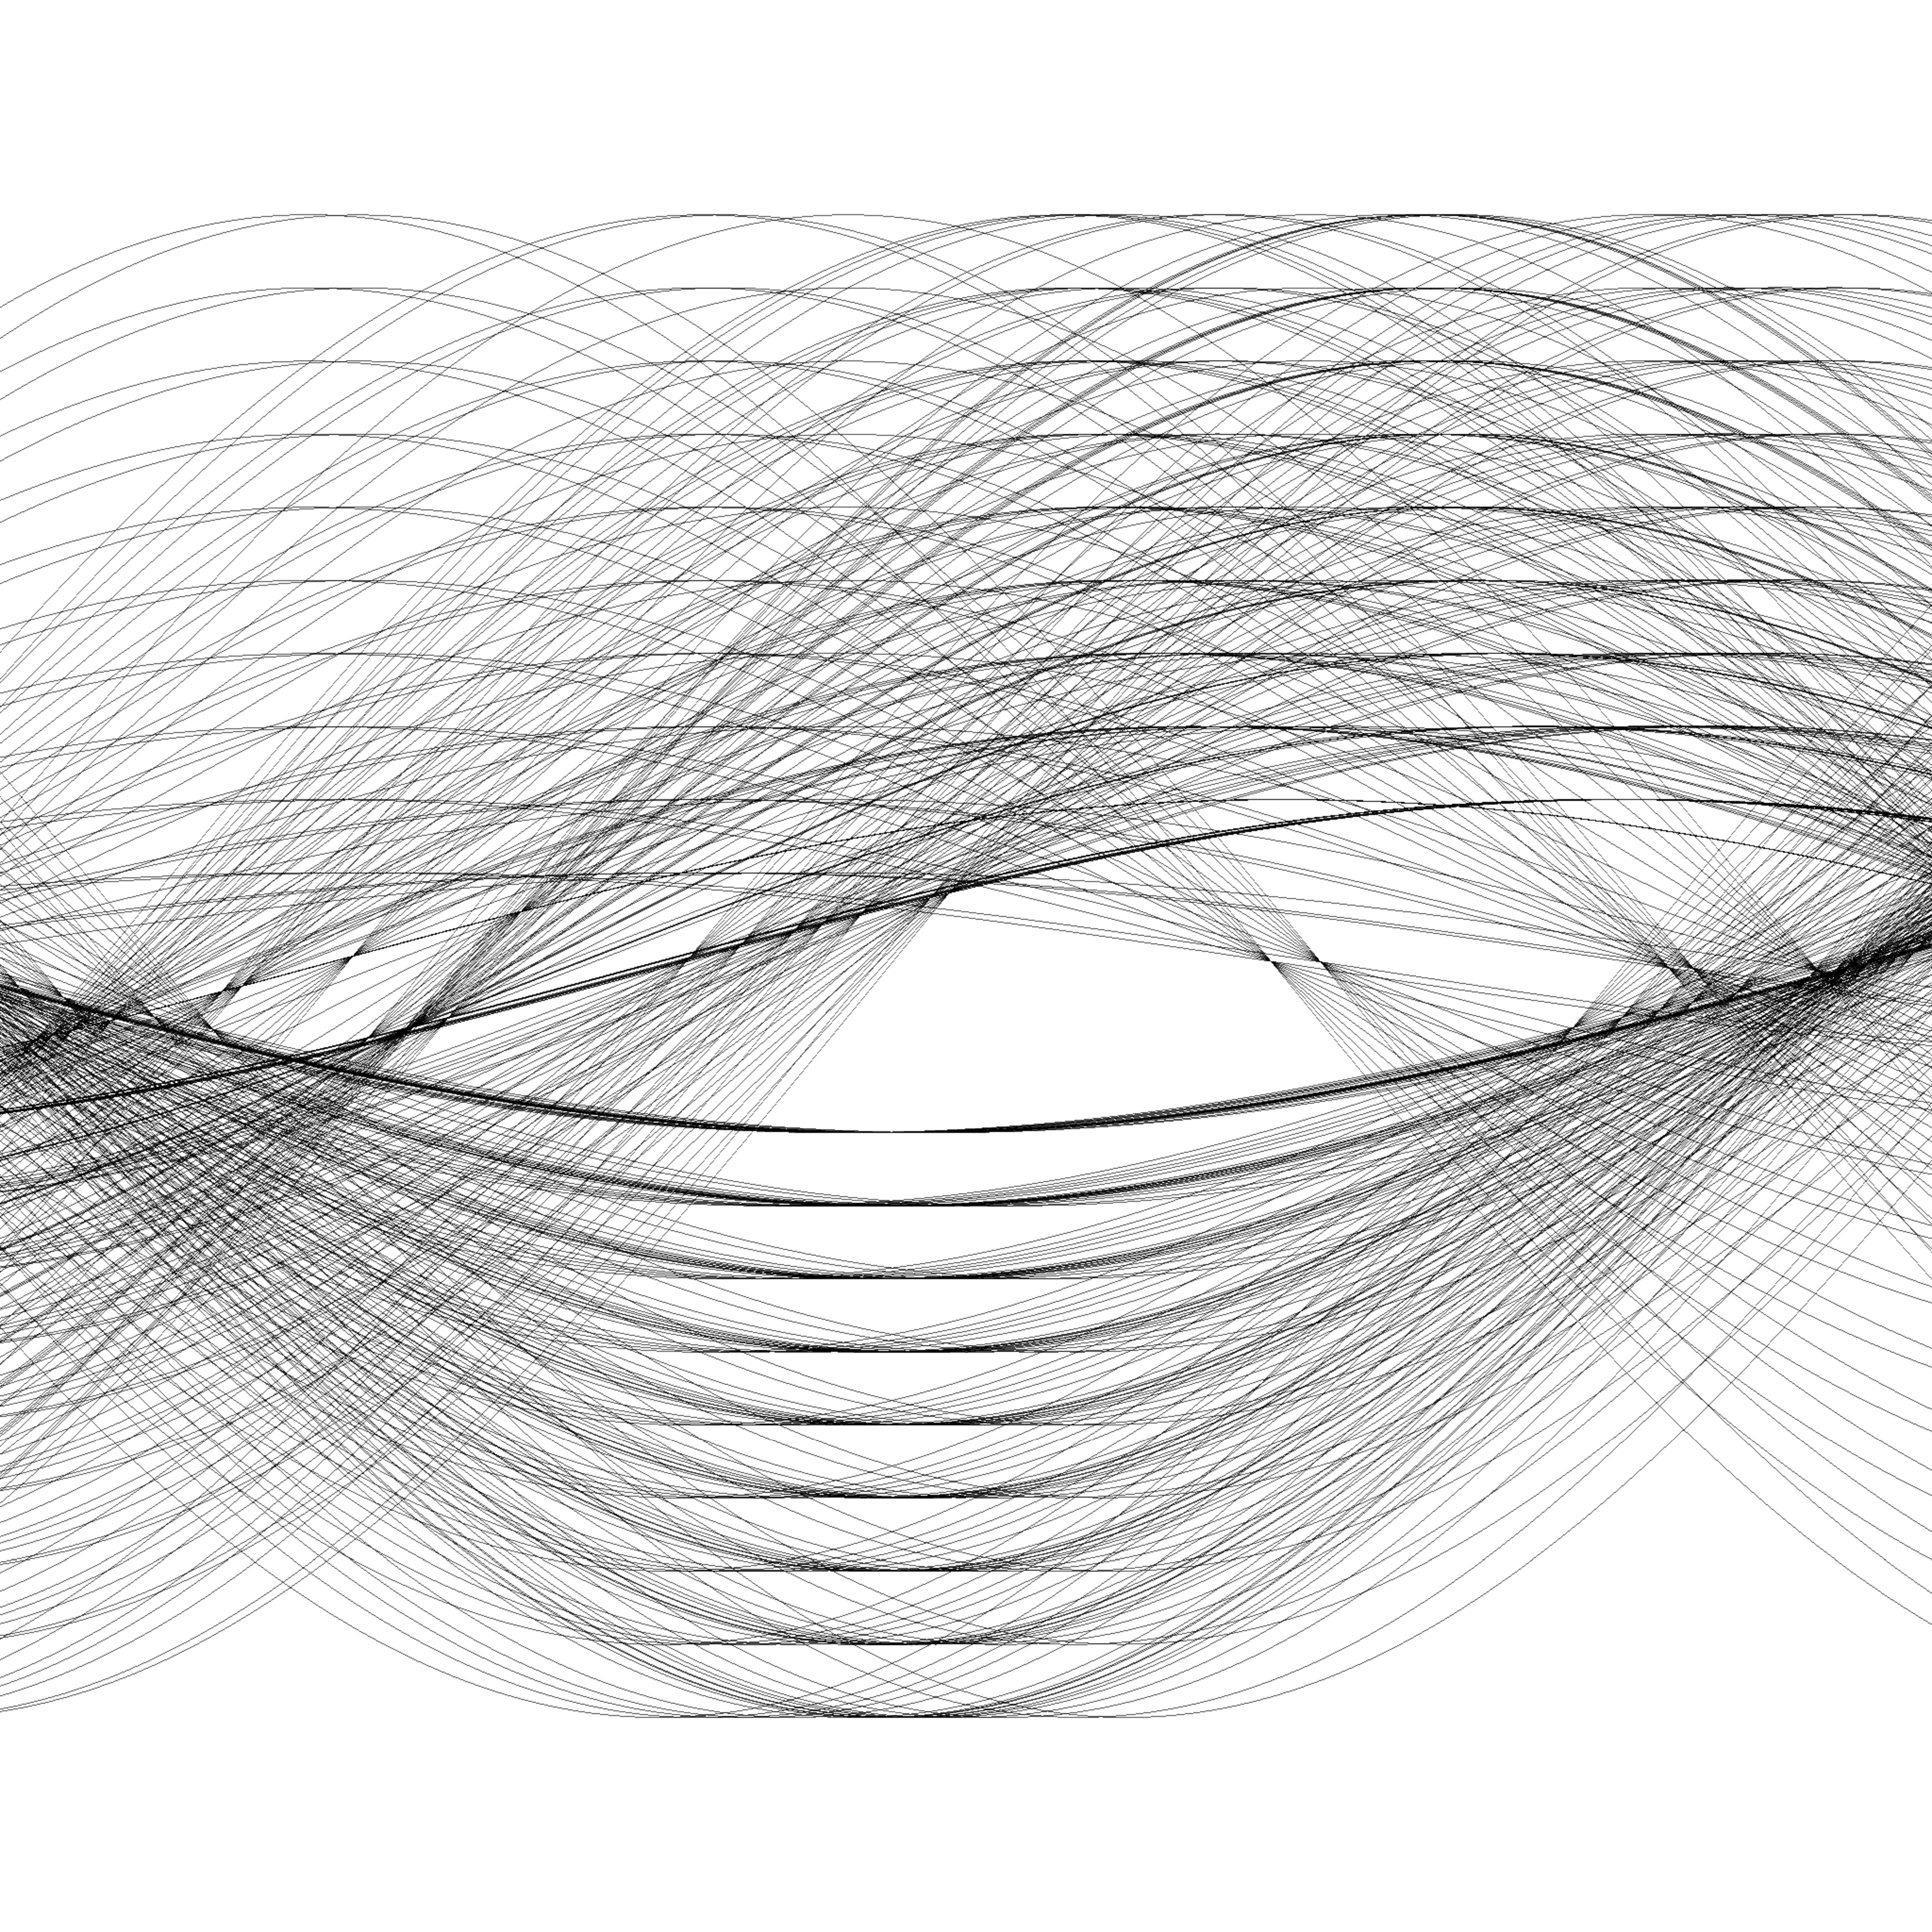
\includegraphics[width=0.30\textwidth]{figs/jet2/accumulator.pdf}
	
\includegraphics[width=0.30\textwidth]{figs/jet2/vertex.pdf}
	\caption{Hough transform algorithm applied to an event with multiple displaced jets. Left: Simulated
	tracks in the event. Center: The parameter space is difficult to visually interpret. Right: The
	second Hough transform identifies the sinusoids corresponding to the jet vertices.
	\label{fig:DisplacedJets}}
\end{center}
\end{figure}

\section{Results}

performance

efficiency (and maybe purity) versus number of tracks at a given singularity

efficiency (and maybe purity) versus total number of singularities

efficiency (and maybe purity) versus distance from interaction point

results with singularities plus normal tracks from the interaction point


\section{Summary}

Improvements have been made on CPU implementation of HT to better quantify relative performance of CPU and GPU implementations.  GPU implementation is still approximately 60x faster than a multithreaded CPU implementation.

Extended usage of HT for detecting new and rare physics phenomena such as displaced jets and black holes.

Massively parallel processor still has advantage in terms of absolute performance.

Further focus on efficiency and/or purity improvements?

Should we do a more formal economic analysis for cost of hardware, operating costs, etc.?  It's hard to account for hardware costs because no one pays retail and lots of sales deals get negotiated.  However, the operating costs could be quantified by plugging computers into power monitors to look at performance per Watt for example.

Would like to investigate performance of Xeon Phi for HT?

\end{document}
